\renewcommand{\nomebreve}{hanoi\_with\_split\_merge}
\renewcommand{\titolo}{Move an Hanoi tower with split and merge moves allowed\\}

\introduzione{}

Studiamo una variante del puzzle della torre di Hanoi. Se non conosci la versione classica o la descrizione quì sotto non basta, sei libero di cercare in internet o sperimentare col seguente applet:

\begin{verbatim}
https://www.mathsisfun.com/games/towerofhanoi.html
\end{verbatim}

Ci sono tre pioli ($A$,$B$ e $C$) su cui sono collocati $n$ dischi numerati da $1$ ad $n$ (dal più piccolo al più grande). Le \emph{configurazioni valide} sono quelle in cui nessun disco si trova collocato sopra un disco più piccolo.
La \emph{configurazione iniziale} è l'unica valida in cui tutti i dischi sono collocati sul piolo $A$. La \emph{configurazione finale} è l'unica valida in cui tutti i dischi sono collocati sul piolo $C$.

\begin{figure}[h!]
\begin{center}
  \noindent 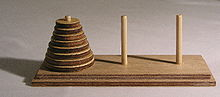
\includegraphics[width=0.57\textwidth]{figures/220px-Tower_of_Hanoi.jpeg}
\end{center}
\caption{Configurazione iniziale $A^8$ del puzzle per $n=8$.}
\end{figure}

Qualsiasi sia il numero di dischi $n$, il tuo obiettivo è quello di portarti dalla configurazione iniziale alla configurazione finale con una sequenza, la più breve possibile, di mosse valide.
Nel puzzle classico offerto da Édouard Lucas (1883) sono consentite solo quelle mosse che spostano un solo disco alla volta, ed è celebre l'elegante soluzione ricorsiva che lo risolve nel minimo numero di mosse. La soluzione ottima è di fatto unica anche se trova diverse descrizioni/rappresentazioni/interpretazioni.

Noi proponiamo di aggiungere le operazioni di \emph{split} e di \emph{merge} al set delle mosse consentite. Pertanto il puzzle ammetterà sicuramente una soluzione che sposta la torre, e noi, tra quelle soluzioni che impiegano il minimo numero di mosse, considereremo \emph{ottime} quelle che ricorrono al minor numero possibile di mosse non-standard (split e merge). Tra queste ve ne è una sola che minimizza il numero di mosse di merge. E' questa la soluzione unica che ti chiediamo di produrre.\\

L'operazione di \emph{split} prevede un piolo sorgente e due pioli destinazione, di cui uno primario. Per un qualche numero naturale $k$, lo split prende gli ultimi (i più piccoli) $k$ dischi collocati sul piolo sorgente e, seguendo il loro ordine, li ripartisce alternativamente sui due pioli destinazione, a cominciare dal disco più grande che finisce sul piolo di destinazione primario. L'operazione viene invocata con una frase del tipo "split il piolo~B, dal disco~5, sui pioli~C e~A", dove 'C' è allora il piolo di destinazione primario e su di esso finisce il disco~5 (il più grande dei dischi spostati).
Ovviamente prima dell'operazione il disco~5 era nel piolo B e vigeva la precondizione che ogni disco eventualemnte presente sul piolo di destinazione primario fosse più grande di~5 (affinchè la configurazione prodotta sia valida). Analoga precondizione vige per l'altro piolo di destinazione, dove ora il disco critico da considerarsi è il secondo disco oggetto della ripartizione.
L'operazione di split si dice \emph{bilanciata} se $k$ è pari, e \emph{sbilanciata} altrimenti. 

L'operazione di \emph{merge} è l'inversa dell'operazione di split, nel senso che la ``disfa'' come andare indietro nel tempo riavvolgendo il nastro alla moviola. Avremo pertanto la categoria delle merge bilanciate (le inverse delle split bilanciate) e quella delle merge sbilanciate (le inverse delle split sbilanciate).
In ogni caso l'operazione di merge potrà essere univocamente individuata da una frase del tipo "merge sul piolo~B, dal disco~5 del piolo~C e dal piolo~A", che inverte precisamente l'invocazione a split riportata sopra, e dove la parte del piolo A interessata resta sempre univocamente individuata (quando il comando è in un qualche modo applicabile). Come per la merge (e per le mosse standard) l'applicabilità non è sempre garantita ma disegue in ultima dal rispetto dalla regola aurea di visitare solo configurazioni valide.

\sezionetesto{Input ed Output}

Per la gestione pulita di input ed output consigliamo di utilizzare il template di soluzione fornito tra gli attachments alla pagina del problema.
Input ed output avvengono da \verb'stdin' e su \verb'stdout' rispettivamente.
La prima ed unica riga dell'input contiene i tre numeri $t$, $t'$ ed $n$, nell'ordine e separati da spazio.
Il parametro $n$ indica il numero di dischi nel puzzle. I parametri $t$ e $t'$ precisano il tipo di richiesta: solo contare ($t=0$) o proprio listare una per una le mosse di una soluzione ottima ($t=1$); senza split e merge ($t'=0$), con split e merge purchè bilanciati ($t'=1$), con split e merge qualsiasi ($t'=2$).

In realtà vogliamo valutare e consentire l'espressione di diverse competenze. Il ruolo del parametro $t$ è pertanto:

\indent
Nel caso in cui $t=0$ il vostro programma deve restituire su \verb'stdout' un unico numero naturale: il minimo numero di mosse che è necessario spendere per portare il gioco nella configurazione finale.

\indent
Nel caso in cui $t= 1$ il vostro programma deve riportare su \verb'stdout' la sequenza ottima di mosse che consente di raggiungere la configurazione finale. Il formato corretto è illustrato negli esempi. Ricordiamo che la soluzione ottima è quella, tra le soluzioni che impiegano il minor numero totale di mosse, a minimizzare poi il numero di mosse non-standard impiegate, e minimizza infine le mosse di merge. Può aiutare pensare che le mosse standard costano 100 ciascuna, quelle di split 110, e quelle di merge 111. Si vuole produrre la soluzione di costo minimo.

Un suggerimento: nel caso $t=1$ l'approccio ricorsivo è fortemente consigliato anche nella stesura del codice, oltre che quando affronti il problema.

L'altro parametro utilizzato per catalogare i subtask è $t'$: se $t'=0$ allora le operazioni di split e merge non sono consentite (puzzle classico), se $t'=1$ allora le sole operazioni di split e merge {\it bilanciate} sono consentite in aggiunta alle mosse standard, se $t'=2$ allora tutte le mosse sopra discusse sono consentite.


% Esempi
\sezionetesto{Esempio di input/output}

In attachment alla pagina del problema trovate diverse coppie input/output tra cui le seguenti.

\vspace{0.5cm}
\esempio{0 0 3}{7}

\vspace{0.5cm}
\esempio{1 0 3}{sposta il disco 1 dal piolo A al piolo C

sposta il disco 2 dal piolo A al piolo B

sposta il disco 1 dal piolo C al piolo B

sposta il disco 3 dal piolo A al piolo C

sposta il disco 1 dal piolo B al piolo A

sposta il disco 2 dal piolo B al piolo C

sposta il disco 1 dal piolo A al piolo C
}

\vspace{0.5cm}
\esempio{0 1 3}{5}

\vspace{0.5cm}
\esempio{1 1 3}{split il piolo A, dal disco 2, sui pioli B e C
  
sposta il disco 1 dal piolo C al piolo B
  
sposta il disco 3 dal piolo A al piolo C

split il piolo B, dal disco 2, sui pioli C e A

sposta il disco 1 dal piolo A al piolo C
}

\vspace{0.5cm}
\esempio{0 2 3}{3}

\vspace{0.5cm}
\esempio{1 2 3}{split il piolo A, dal disco 3, sui pioli C e B

sposta il disco 1 dal piolo C al piolo A

merge sul piolo C, dal disco 2 del piolo B e dal piolo A
}


\section*{Subtask}

  \begin{itemize}
    \item \textbf{Subtask 1 [0 punti]:} i casi di esempio forniti alla pagina del problema, essi includono i sei casi sopra.
    \item \textbf{Subtask 2 [5 punti]:} $t=0$, $t'=0$, $n \le 30$.
    \item \textbf{Subtask 3 [5 punti]:} $t=1$, $t'=0$, $n \le 15$.
      
    \item \textbf{Subtask 4 [12 punti]:} $t=0$, $t'=1$, $n \le 30$.
    \item \textbf{Subtask 5 [12 punti]:} $t=1$, $t'=1$, $n \le 15$.
    \item \textbf{Subtask 6 [13 punti]:} $t=0$, $t'=1$, $n \le 100$.
    \item \textbf{Subtask 7 [13 punti]:} $t=1$, $t'=1$, $n \le 100$.
      
    \item \textbf{Subtask 8 [10 punti]:} $t=0$, $t'=2$, $n \le 30$.
    \item \textbf{Subtask 9 [10 punti]:} $t=1$, $t'=2$, $n \le 15$.
    \item \textbf{Subtask 10 [10 punti]:} $t=0$, $t'=2$, $n \le 100$.
    \item \textbf{Subtask 11 [10 punti]:} $t=1$, $t'=2$, $n \le 100$.
  \end{itemize}
  
